\begin{figure}[!htb]
    \centering
    \tikzstyle{every node}=[font=\large]
    
    \tikzstyle{task} = [rectangle, rounded corners, minimum width=4cm, minimum height=1.5cm,text centered, draw=black, fill=white!30, text width=3.5cm, font=\large]
    \tikzstyle{phase} = [rectangle, minimum width=4cm, minimum height=1.5cm,text centered, draw=black, fill=white!30, text width=3.5cm, font=\Large]
    \tikzstyle{--} = [black, line width = 2mm]
    \tikzstyle{--red} = [ccmRed, rounded corners, line width = 2mm]
    \tikzstyle{arrow_blue} = [ccmDBlue, rounded corners, line width = 2mm, ->]
    \tikzstyle{arrow_red} = [ccmRed, rounded corners, line width = 2mm, ->]
    
    
    \setlength{\fboxsep}{0pt}%
    \setlength{\fboxrule}{1mm}

    \resizebox{\linewidth}{!}{
    \begin{tikzpicture}[node distance=1cm]
        
        \node (image1) [] {\fbox{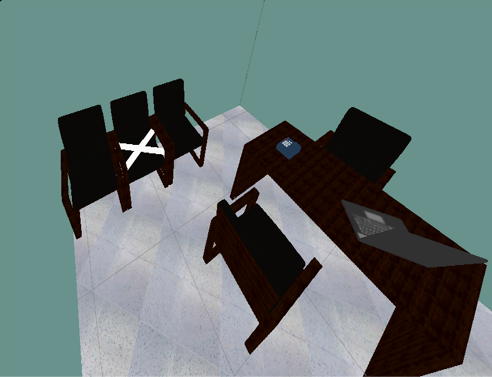
\includegraphics[width = 0.5\linewidth]{Metodologia/VE.png}}};
        \node (image2) [right of = image1, xshift = 7.15cm] {\fbox{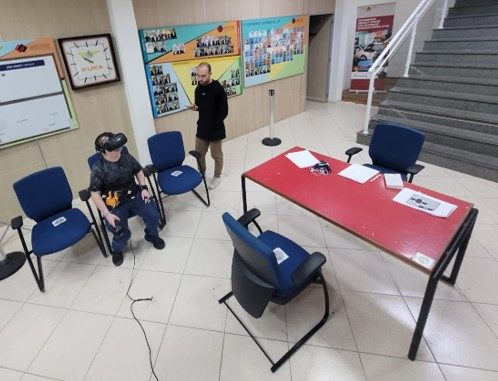
\includegraphics[width = 0.5\linewidth]{Metodologia/RE.jpg}}};

        \node (image3) [below of = image1, yshift = -10cm] {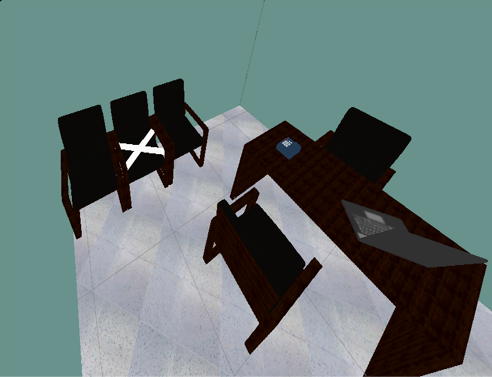
\includegraphics[width = 0.5\linewidth]{Metodologia/VE.png}};
        \node (image4) [right of = image3, xshift = 7.15cm] {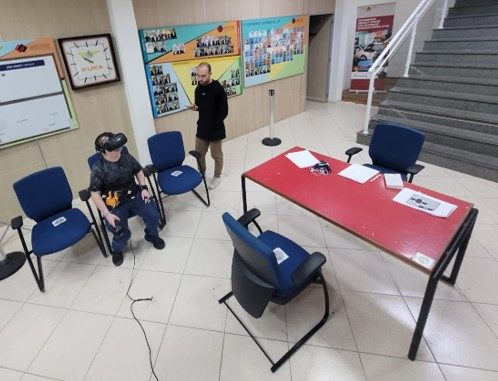
\includegraphics[width = 0.5\linewidth]{Metodologia/RE.jpg}};

        %\node (ponto1) [above of = image1, yshift = 2.5cm, left of = image1, xshift = -3cm] {};
        %\node (ponto2) [above of = image1, yshift = 2.5cm, right of = image1, xshift = 3cm]{};
    
        %\draw[--] (ponto1.west) -- (ponto2.east);
        
    \end{tikzpicture}
    }
    \caption{Virtual and Real environment comparisson}
    \label{fig:ve_re}
\end{figure}